\section{齐次方程齐次边界条件}
\label{sec:homo}
本节先讨论齐次方程及齐次边界条件的定解问题,

% 本节先讨论齐次方程及齐次边界条件的定解问题, 随后讨论对非齐次方程及非齐次边界条件的处理,最后讨论高维的情形.

% \subsection{齐次方程及齐次边界条件的定解问题}
我们通过实例说明用分离变量法解题的六个基本步骤.

% \begin{examplebox}{求两端固定的弦自由振动的规律.}

求两端固定的弦自由振动的规律.
定解问题为
\begin{equation}
    \begin{cases}u_{t t}-a^{2} u_{x x}=0, & 0<x<l, \quad t>0 
        \\ u(0, t)=0, \quad u(l, t)=0 & 
        \\ u(x, 0)=\varphi(x), \quad u_{t}(x, 0)=\psi(x) & 
    \end{cases}
    \label{eq:string_vibration_equation}
\end{equation}

\begin{enumerate}
  \item \textbf{分离变量}

    令
    \begin{equation}
        u(x, t)=X(x) T(t)
        \label{eq:uxt}
    \end{equation}
    将式\eqref{eq:uxt}代入泛定方程\eqref{eq:string_vibration_equation}, 可得
    $$
    X(x) T^{\prime \prime}(t)-a^{2} X^{\prime \prime}(x) T(t)=0
    $$
即
$$
\frac{X^{\prime \prime}(x)}{X(x)}=\frac{T^{\prime \prime}(t)}{a^{2} T(t)}
$$

由于上式右端与 $x$ 无关,左端与 $t$ 无关, 而 $x$ 与 $t$ 又是互相独立的变量, 
因此上式只有等于常数才能成立. 令常数为 $-\lambda$, 便得到两个常微分方程
\begin{equation}
    \begin{aligned}
        & X^{\prime \prime}(x)+\lambda X(x)=0 \\
        & T^{\prime \prime}(t)+\lambda a^{2} T(t)=0
        \end{aligned}
        \label{eq:XT}
\end{equation}

将式\eqref{eq:uxt}代入边界条件, 可得
$$
u(0, t)=X(0) T(t)=0, \quad u(l, t)=X(l) T(t)=0
$$
若 $T(t)=0$, 代入式\eqref{eq:uxt} 得 $u(x, t)=0$, 是平庸解, 应略去. 由此得边界条件
\begin{equation}
    X(0)=0, \quad X(l)=0
    \label{eq:boundary}
\end{equation}

\item \textbf{求解本征值问题}

式\eqref{eq:XT}及式\eqref{eq:boundary}构成了常微分方程的边值问题
$$
\left\{\begin{array}{l}
X^{\prime \prime}(x)+\lambda X(x)=0 \\
X(0)=0, \quad X(l)=0
\end{array}\right.
$$
这称为本征值问题. 
可以证明, 只有当 $\lambda$ 取某些特定值时才有非零解,
求解本征值问题就是求解本征值 $\lambda$ 与本征函数 $X(x)$.

现将 $\lambda$ 的取值分三种情况讨论:

\begin{itemize}
    \item 若 $\lambda<0$, 这时方程的通解为 $X(x)=A e^{\sqrt{-\lambda} x}+B e^{-\sqrt{-\lambda} x}$.

        由边界条件 $X(0)=X(l)=0$, 可得
        
        $$
        \left\{\begin{array}{l}
        A+B=0 \\
        A e^{\sqrt{-\lambda l}}+B e^{-\sqrt{-\lambda l}}=0
        \end{array}\right.
        $$
        
        这是关于 $A 、 B$ 的线性齐次方程组, 由于系数行列式不为零, 故 $A=B=0$. 因此 $\lambda<0$ 时, $X(x)$ 无非零解.

    \item 若 $\lambda=0$, 这时方程成为 $X^{\prime \prime}(x)=0$, 它的通解为 $X(x)=A x+B$.

        由边界条件 $X(0)=X(l)=0$ 得 $A=B=0, X(x)$ 也无非零解.
    
    \item 若 $\lambda>0$, 方程的通解为 $X(x)=A \cos \sqrt{\lambda} x+B \sin \sqrt{\lambda} x$.

        由边界条件 $X(0)=0$, 得 $A=0$. 由 $X(l)=0$ 得 $B \sin \sqrt{\lambda} l=0$. 非零解要求 $B \neq 0$, 故
        
        $$
        \sin \sqrt{\lambda} l=0 \quad \text { 即 } \sqrt{\lambda}=\frac{n \pi}{l}, \quad n=1,2, \cdots
        $$
        
        因此本征值 (加上脚标 $n$ ) 及相应的本征函数分别为
        
        $$
        \lambda_{n}=\left(\frac{n \pi}{l}\right)^{2}, \quad n=1,2, \cdots
        $$
        
        $$
        X_{n}(x)=B_{n} \sin \frac{n \pi x}{l}, \quad n=1,2, \cdots
        $$
\end{itemize}





  \item \textbf{求解 $T(t)$ 的常微分方程}
  
    将本征值 $\lambda_{n}=\left(\frac{n \pi}{l}\right)^{2}$ 代入式\eqref{eq:XT}, 得到

    $$
    T^{\prime \prime}(t)+\left(\frac{n \pi a}{l}\right)^{2} T(t)=0
    $$

    它的通解为
    $$
    T_{n}(t)=C_{n} \cos \frac{n \pi a t}{l}+D_{n} \sin \frac{n \pi a t}{l}
    $$
    式中 $C_{n}$ 和 $D_{n}$ 为任意常数.
    
    \item \textbf{作特解的线性叠加}
    
    满足方程及边界条件\eqref{eq:string_vibration_equation}的一系列特解为
    \begin{equation}
        u_{n}(x, t)=X_{n}(x) T_{n}(t)=\left(C_{n} \cos \frac{n \pi a t}{l}+D_{n} \sin \frac{n \pi a t}{l}\right) \sin \frac{n \pi x}{l}, 
        \label{eq:special_solution}
    \end{equation}
    这里已将任意常数 $B_{n}$ 吸收到任意常数 $C_{n}$ 及 $D_{n}$ 中去了.
    
    特解\eqref{eq:special_solution}一般不满足初始条件, 实际上由式\eqref{eq:special_solution}可得 
    $$
    \begin{aligned}
    u_{n}(x, 0) & =C_{n} \sin \frac{n \pi x}{l} \\
    \left.\frac{\partial u_{n}(x, t)}{\partial t}\right|_{t=0} & =D_{n} \frac{n \pi a}{l} \sin \frac{n \pi x}{l}
    \end{aligned}
    $$

    这表明, 除非 $\varphi(x)$ 和 $\psi(x)$ 同时为 $\sin \frac{n \pi x}{l}$ 的倍数,
     否则任何一个特解不可能满足题目给定的初始条件. 
     但考虑到方程  及边界条件\eqref{eq:string_vibration_equation}都是齐次线性的, 
     因此将所有的特解线性叠加起来, 如果级数收玫, $u(x, t)$ 仍然满足方程 与边界条件. 由此得
    \begin{equation}
        u(x, t)=\sum_{n=1}^{\infty} u_{n}(x, t)=
        \sum_{n=1}^{\infty}\left(C_{n} \cos \frac{n \pi a t}{l}+
        D_{n} \sin \frac{n \pi a t}{l}\right) \sin \frac{n \pi x}{l}
        \label{eq:general_solution}
    \end{equation}
    而待定系数 $C_{n}$ 和 $D_{n}$ 可由初始条件来确定.
    

    \item \textbf{由初始条件确定系数} 
    
        将式\eqref{eq:general_solution}代入初始条件, 即有
        $$
        \begin{gathered}
        \varphi(x)=u(x, 0)=\sum_{n=1}^{\infty} C_{n} \sin \frac{n \pi x}{l} \\
        \psi(x)=u_{t}(x, 0)=\sum_{n=1}^{\infty} D_{n} \frac{n \pi a}{l} \sin \frac{n \pi x}{l}
        \end{gathered}
        $$
        最终系数可由前面傅里叶级数展开来确定系数$C_{n}$ 及 $D_{n}$, 即得定解问题的解.
        $$
        \begin{aligned}
        & C_{n}=\frac{2}{l} \int_{0}^{l} \varphi(x) \sin \frac{n \pi x}{l} d x, \quad n=1,2, \cdots \\
        & D_{n}=\frac{2}{n \pi a} \int_{0}^{l} \psi(x) \sin \frac{n \pi x}{l} d x, \quad n=1,2, \cdots
        \end{aligned}
        $$


        \item \textbf{解的物理意义}
        
        先看级数\eqref{eq:general_solution} 的每一项 (即每一个特解)的物理意义.

        \begin{equation}
            u_{n}(x, t)=\left(C_{n} \cos \frac{n \pi a t}{l}+D_{n} \sin \frac{n \pi a t}{l}\right) \sin \frac{n \pi x}{l}
            =E_{n} \cos \left(\omega_{n} t-\varphi_{n}\right) \sin \frac{n \pi x}{l}
            \label{eq:solution_2}
        \end{equation}    
        式中
        $$
        E_{n}=\sqrt{C_{n}^{2}+D_{n}^{2}}, 
            \quad \omega_{n}=\frac{n \pi a}{l}, 
            \quad \varphi_{n}=\tan ^{-1} \frac{D_{n}}{C_{n}}
        $$
        
        如果弦按式\eqref{eq:solution_2}的规律运动时, 
        $x=0$ 及 $x=l$ 这两个端点保持不动. 
        而弦上各点则在各自的平衡位置附近作简谐振动, 
        其振幅分别为 $E_{n}\left|\sin \frac{n \pi x}{l}\right|$. 
        弦的这种形式的运动称为\textbf{驻波}. 
        在点 $x=\frac{m l}{n}(m=0,1, \cdots, n)$ 处, 振幅为零. 
        这些点在整个振动过程中始终保持不动, 称为驻波 $u_{n}(x, t)$ 的\textbf{波节}. 
        在点 $x=\frac{2 m+1}{2 n} l(m=0,1$, $\cdots, n-1)$ 处, 
        $\sin \frac{n \pi x}{l}= \pm 1$, 这些点的振幅最大,称为驻波的\textbf{波腹}.
         驻波的\textbf{角频率} $\omega_{n}=\frac{n \pi}{l}$, 
         其中 $n=1$ 的项 $u_{1}(x, t)$ 称为\textbf{基波}, 
         而 $n>1$ 的项 $u_{n}(x, t)$ 称为 \textbf{$n$ 次谐波}, 
         这些驻波也称为两端固定弦的本征振动. 
         因此, 有界弦的任意振动可看作一系列本征振动的叠加.
        
\end{enumerate}



\setlength\intextsep{5pt}
下一个例题是平面极坐标系的分离变数法.

带电的云跟大地之间的静电场近似是匀强静电场, 其电场强度 $\bE_{0}$
是坚直的. 水平架设的输电线处在这个静电场之中(图\ref{fig:wire}). 
输电线是导体圆柱. 柱面由于静电感应出现感应电荷, 圆柱邻近的静电场也就不再是匀强的了. 
不过, 离圆柱 “无限远” 处的静电场仍保持为匀强的. 
现在研究导体圆柱怎样改变了匀强静电场.
\begin{wrapfigure}{r}{0.3\textwidth}
    \begin{center}
        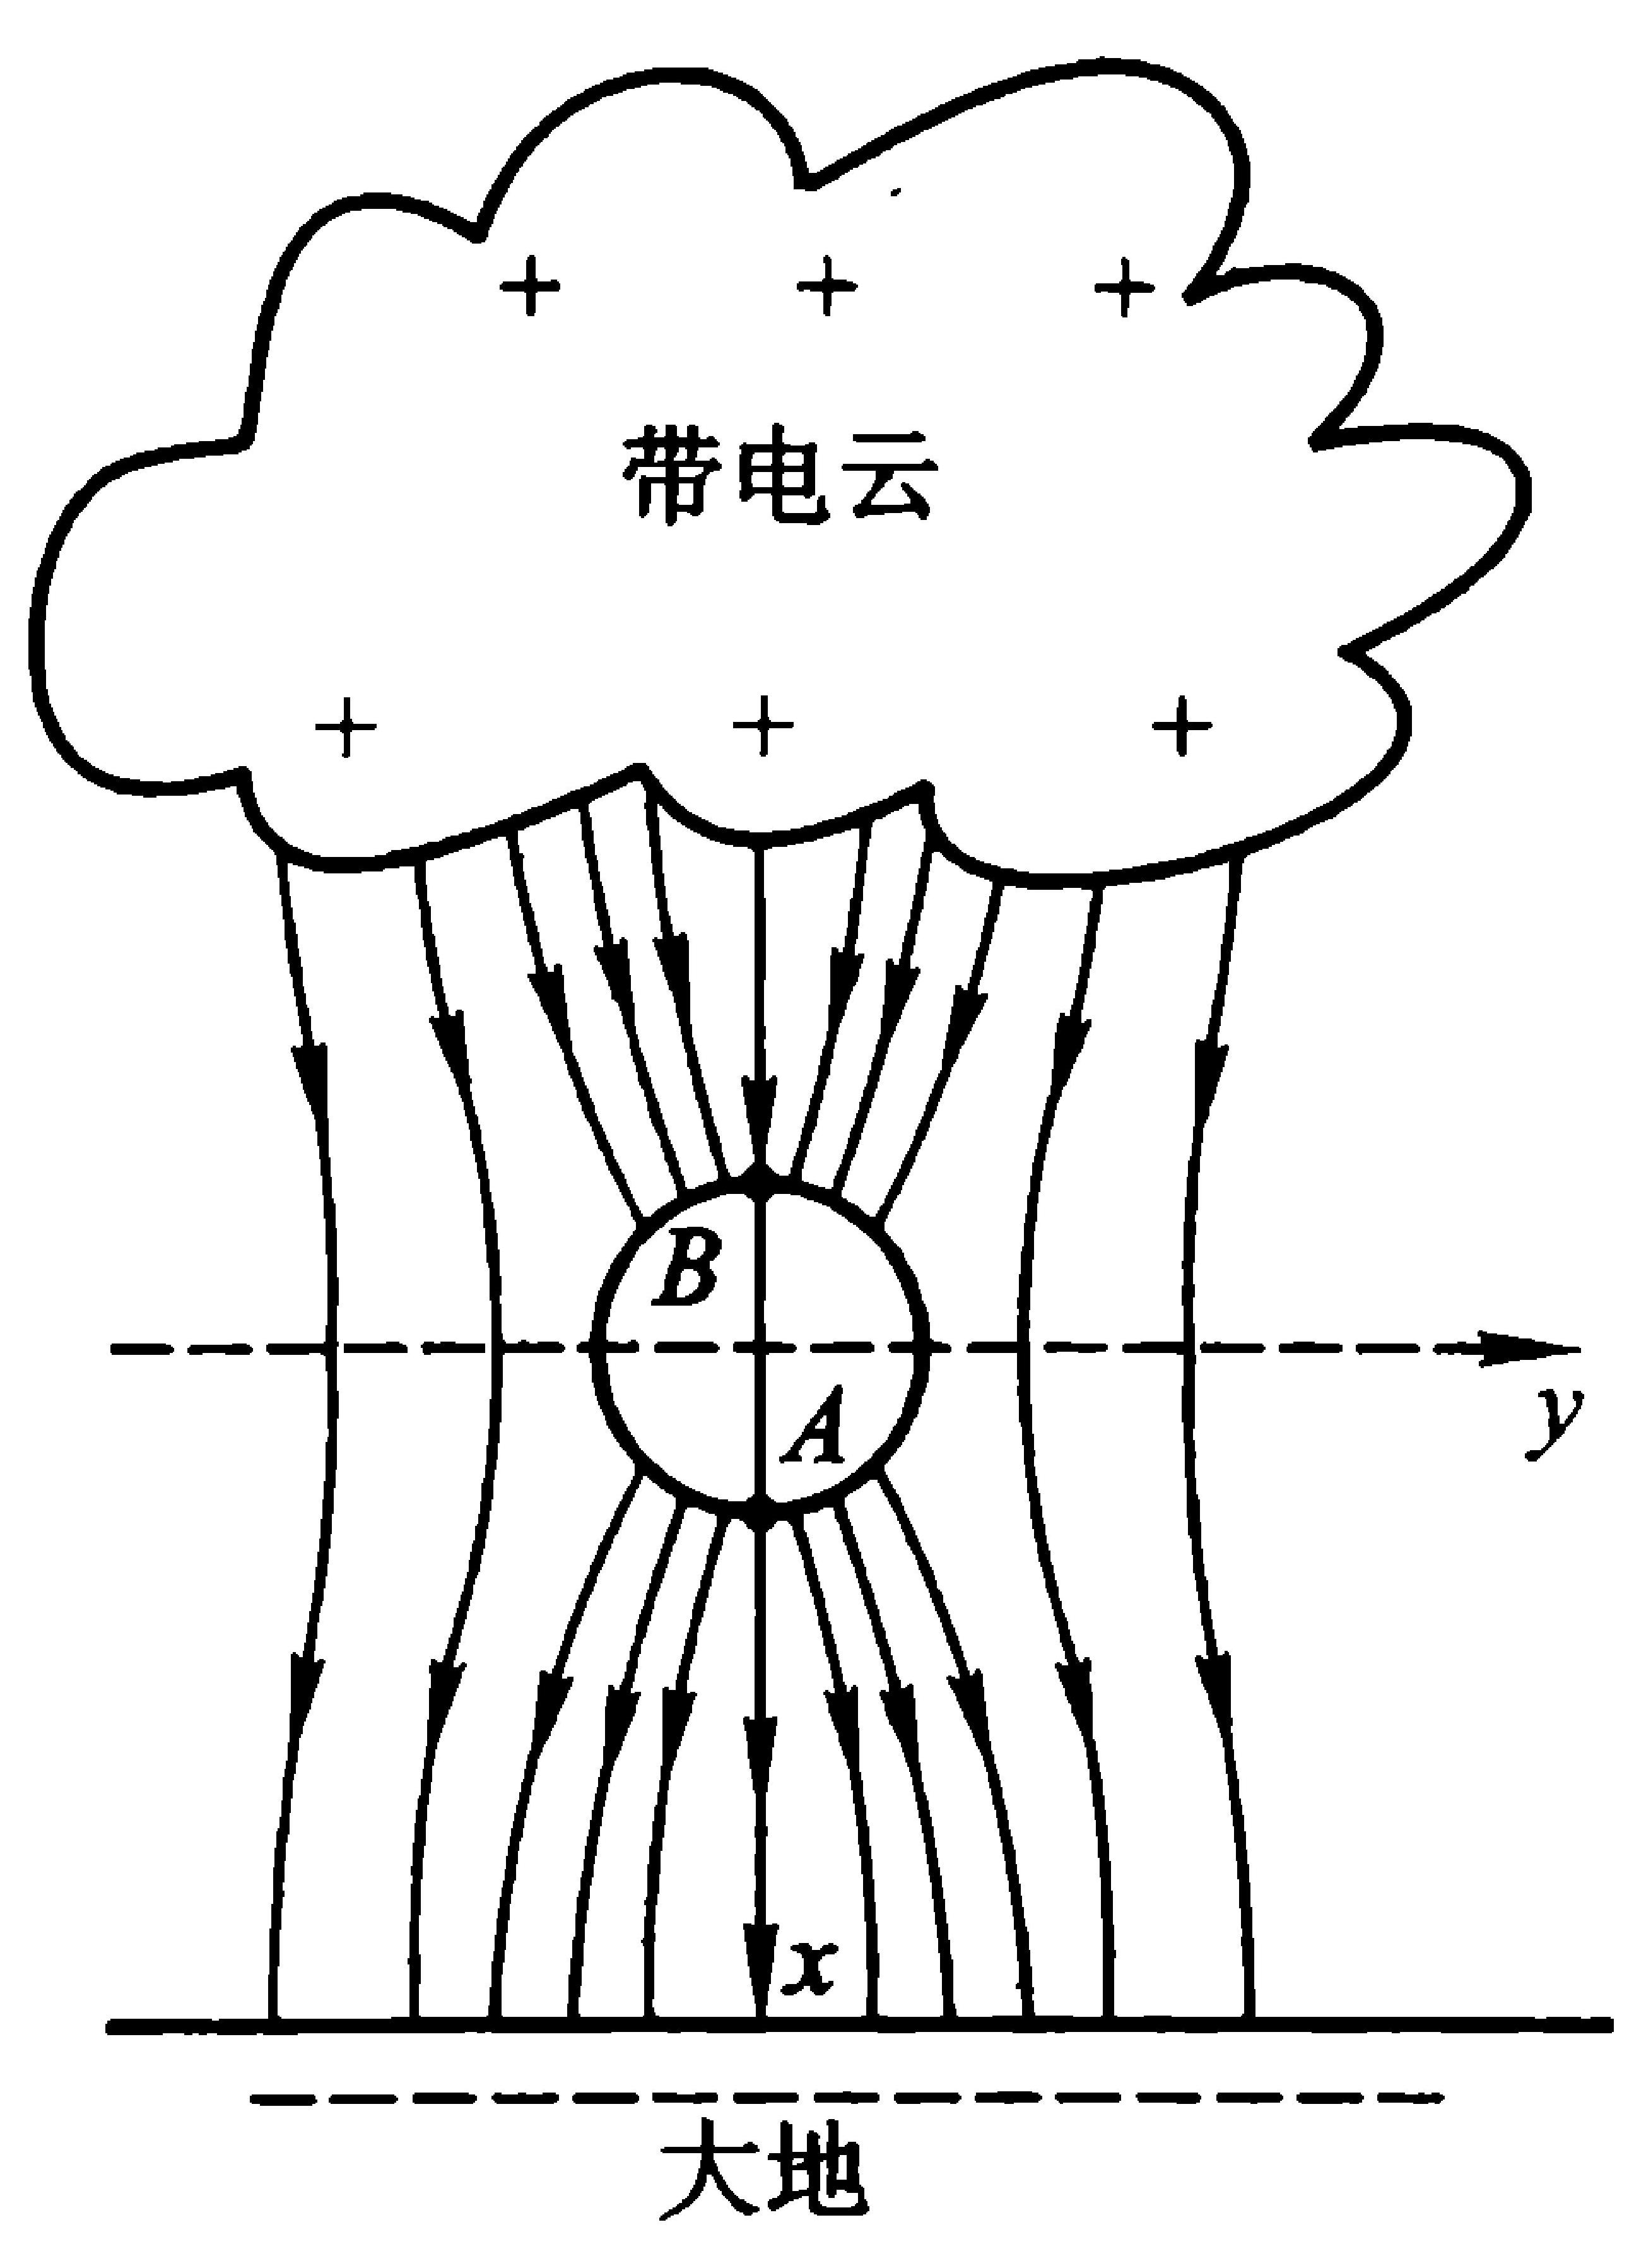
\includegraphics[width=0.3\textwidth]{wire.jpg}
    \end{center}
    \vspace{-20pt}
    \caption{输电线示意图.}
    \vspace{-10pt}
    \label{fig:wire}
  \end{wrapfigure}
首先需要把这个物理问题表为定解问题. 取圆柱的轴为 $z$ 轴. 
如果圆柱 “无限长”, 那么, 这个静电场的电场强度、电势显然跟 $z$ 无关, 我们只需在 $x y$ 平面上加以研究就够了.
图\ref{fig:wire}画的正是 $xy$ 平面上的静电场, 圆柱面在
$xy$ 平面的剖口是圆 $x^{2}+y^{2}=a^{2}$, 其中 $a$ 是圆柱的半径.

柱外的空间中没有电荷, 所以电势 $u$ 满足二维的拉普拉斯方程

$$
u_{x x}+u_{y y}=0 \quad \text { (柱外). }
$$

导体中的电荷既然不再移动, 这说明导体中各处电势相同. 又因为电势只具有相对的意义, 不妨把电势的零点取在导体上, 从而写出边界条件

$$
\left.u\right|_{x^{2}+y^{2}=a^{2}}=0 .
$$

按照分离变数法, 以 $u(x, y)=X(x) Y(y)$ 代入拉普拉斯方程固然不难把它分解为两个常微分方程,但代入上述边界条件却只能得到

$$
X(x) Y\left(\sqrt{a^{2}-x^{2}}\right)=0
$$
不能分解为 $X(x)$ 或 $Y(y)$ 的边界条件. 事实上, 既然边界是圆, 直角坐标系显然是不适当的, 必须采用平面极坐标系.

“柱外空间中的电势 $u$ 满足拉普拉斯方程” 就表为
\begin{equation}
    \frac{\partial^{2} u}{\partial \rho^{2}}+\frac{1}{\rho} \frac{\partial u}{\partial \rho}+
    \frac{1}{\rho^{2}} \frac{\partial^{2} u}{\partial \varphi^{2}}=0 \quad(\rho>a)
    \label{eq:laplace_2d}
\end{equation}
式中 $\rho$ 是极径, $\varphi$ 是极角. “导体电势为零” 就表为齐次的边界条件
\begin{equation}
    \left.u\right|_{\rho=a}=0 .
    \label{eq:laplace_2d_bc}
\end{equation}


在 “无限远” 处的静电场仍然保持为匀强的 $\bE_{0}$. 由于选取了 $x$ 轴平行于 
$\bE_{0}$, 所以在无限远处, $E_{y}=0, E_{x}=E_{0}$, 即 $-\partial u / \partial x=E_{0}$, 
亦即 $u=-E_{0} x=$ $-E_{0} \rho \cos \varphi$. 另外, 导体圆柱还可能带电, 
若单位长度导体带的电量为 $q_{0}$, 它在圆柱外产生的电势为 $\left(q_{0} / 2 \pi \varepsilon_{0}\right) \ln (1 / \rho)$, 
因而还有一个非齐次的边界条件

\begin{equation}
    \left.u\right|_{\rho \rightarrow \infty} \sim u_{0}+
    \frac{q_{0}}{2 \pi \varepsilon_{0}} \ln \frac{1}{\rho}-E_{0} \rho \cos \varphi
    \label{eq:u_rho_infty}
\end{equation}
其中 $u_{0}$ 为常数, 其数值跟电势的零点选取有关. 这里要求其满足在圆柱导体侧面上电势为零. 
问题归结为求解平面极坐标系定解问题 \eqref{eq:laplace_2d}, \eqref{eq:laplace_2d_bc}.

按照前面的步骤, 以分离变数形式的试探解
$$
u(\rho, \varphi)=R(\rho) \Phi\left(\varphi\right)
$$
代入拉普拉斯方程\eqref{eq:laplace_2d}, 得
$$
\frac{\rho}{R} \cdot \frac{d}{d \rho}\left(\rho \frac{d R}{d \rho}\right)=-\frac{\Phi^{\prime \prime}}{\Phi}
$$

上式左边是 $\rho$ 的函数,与 $\varphi$ 无关; 右边是 $\varphi$ 的函数,与 $\rho$ 无关.
 两边不可能相等, 除非两边实际上是同一个常数. 把这常数记作 $\lambda$,

$$
-\frac{\Phi^{\prime \prime}}{\Phi}=\lambda=\frac{\rho}{R} \cdot \frac{d}{d \rho}\left(\rho \frac{d R}{d \rho}\right)
$$

这就分解为两个常微分方程

\begin{eqnarray}
        \Phi^{\prime \prime}+\lambda \Phi &=& 0, \\
        \label{eq:Phi}
        \rho^{2} R^{\prime \prime}+\rho R^{'}-\lambda R  &=& 0.
        \label{eq:R}
\end{eqnarray}
常微分方程\eqref{eq:Phi}隐含着一个附加条件. 
事实上, 一个确定地点的极角可以加减 $2 \pi$ 的整倍数, 而电势 $u$ 在确定的地点应具确定数值, 
所以 $u(\rho, \varphi$ $+2 \pi)=u(\rho, \varphi)$ , 
即 $R(\rho) \Phi(\varphi+2 \pi)=R(\rho) \Phi(\varphi)$ ,亦即
\begin{equation}
    \Phi(\varphi+2 \pi)=\Phi(\varphi)
    \label{eq:Phi_bc}
\end{equation}
这叫做自然的周期条件. 常微分方程\eqref{eq:Phi} 与条件\eqref{eq:Phi_bc} 构成本征值问题. 
同样取 $\lambda$ 为实数, 不难求得方程的解为
\begin{equation}
\Phi(\varphi)= 
    \begin{cases}
        A \cos \sqrt{\lambda} \varphi+B \sin \sqrt{\lambda} \varphi & (\lambda>0), 
        \\ 
        A+B \varphi & (\lambda=0), 
        \\ 
        A e^{\sqrt{-\lambda \varphi}}+B e^{-\sqrt{-\lambda \varphi}} & (\lambda<0) .
    \end{cases}
\end{equation}

从而, 求得本征值
\begin{equation}
    \lambda =m^{2} \quad(m=0,1,2, \cdots) ; \\
    \label{eq:Phi_ev}
\end{equation}
和本征函数
\begin{equation}
\Phi(\varphi) = \begin{cases}A \cos m \varphi+B \sin m \varphi & (m \neq 0), \\
A & (m=0)\end{cases}
\label{eq:Phi_ef}
\end{equation}
以本征值\eqref{eq:Phi_ev}代入常微分方程\eqref{eq:R},
$$
\rho^{2} \frac{d^{2} R}{d \rho^{2}}+\rho \frac{d R}{d \rho}-m^{2} R=0
$$

这是欧拉型常微分方程, 作代换 $\rho=e^{t}$, 即 $t=\ln \rho$, 方程化为
$$
\frac{d^{2} R}{d t^{2}}-m^{2} R=0
$$
其解为

$$
R(\rho)= \begin{cases}C e^{m t}+D e^{-m t}=C \rho^{m}+D \frac{1}{\rho^{m}} & (m \neq 0) \\ C+D t=C+D \ln \rho & (m=0)\end{cases}
$$

这样, 分离变数形式的本征解是

$$
\begin{gathered}
u_{0}(\rho, \varphi)=C_{0}+D_{0} \ln \rho \\
u_{m}(\rho, \varphi)=\rho^{m}\left(A_{m} \cos m \varphi+B_{m} \sin m \varphi\right)+\rho^{-m}\left(C_{m} \cos m \varphi+D_{m} \sin m \varphi\right)
\end{gathered}
$$

拉普拉斯方程是线性的, 它的一般解应是所有本征解的叠加, 即

\begin{equation}
\begin{aligned}
u(\rho, \varphi)= & C_{0}+D_{0} \ln \rho+\sum_{m=1}^{\infty} \rho^{m}\left(A_{m} \cos m \varphi+B_{m} \sin m \varphi\right) \\
& +\sum_{m=1}^{\infty} \rho^{-m}\left(C_{m} \cos m \varphi+D_{m} \sin m \varphi\right)
\end{aligned}
\label{eq:u_rho_phi_general}
\end{equation}

为确定\eqref{eq:u_rho_phi_general} 中的系数, 把它代入边界条件. 先代入齐次边界条件\eqref{eq:laplace_2d_bc},
$$
\begin{gathered}
C_{0}+D_{0} \ln a+\sum_{m=1}^{\infty} a^{m}\left(A_{m} \cos m \varphi+B_{m} \sin m \varphi\right) \\
+\sum_{m=1}^{\infty} a^{-m}\left(C_{m} \cos m \varphi+D_{m} \sin m \varphi\right)=0
\end{gathered}
$$
一个傅里叶级数等于零, 意味着所有傅里叶系数为零, 即
$$
C_{0}+D_{0} \ln a=0, \quad a^{m} A_{m}+a^{-m} C_{m}=0, \quad a^{m} B_{m}+a^{-m} D_{m}=0
$$
由此,

$$
C_{0}=-D_{0} \ln a, \quad C_{m}=-A_{m} a^{2 m}, \quad D_{m}=-B_{m} a^{2 m}
$$

以此代入\eqref{eq:u_rho_phi_general}, 得
\begin{equation}
    \begin{aligned}
        u(\rho, \varphi)= & D_{0} \ln \frac{\rho}{a}+\sum_{m=1}^{\infty} \rho^{m}\left(A_{m} \cos m \varphi+B_{m} \sin m \varphi\right) \\
        & +\sum_{m=1}^{\infty} \rho^{-m}\left(-a^{2 m} A_{m} \cos m \varphi-a^{2 m} B_{m} \sin m \varphi\right)
        \end{aligned}
        \label{eq:u_rho_phi_2}
\end{equation}


将 \eqref{eq:u_rho_phi_2} 代入非齐次的边界条件\eqref{eq:u_rho_infty}, 在 $\rho$ 很大的地方, 有
\begin{equation}
    \begin{gathered}
        D_{0} \ln \frac{\rho}{a}+\sum_{m=1}^{\infty}\left[A_{m}\left(\rho^{m}-\frac{a^{2 m}}{\rho^{m}}\right) \cos m \varphi+B_{m}\left(\rho^{m}-\frac{a^{2 m}}{\rho^{m}}\right) \sin m \varphi\right] \\
        \sim u_{0}+\frac{q_{0}}{2 \pi \varepsilon_{0}} \ln \frac{1}{\rho}-E_{0} \rho \cos \varphi
    \end{gathered}
    \label{eq:matching}
\end{equation}
既然主要部分是 $\rho^{1}$ 项, 可见上式中不应出现 $\rho^{m}(m>1)$ 的项 (否则 $\rho^{m}$ 项就成了主要部分)。这是说,
$$
A_{m}=0, B_{m}=0 . \quad(m>1)
$$

从\eqref{eq:matching}比较系数, 还能知道
$$
B_{1}=0, A_{1}=-E_{0}, D_{0}=-\frac{q_{0}}{2 \pi \varepsilon_{0}}, 
u_{0}=-D_{0} \ln a=\frac{q_{0}}{2 \pi \varepsilon_{0}} \ln a
$$
最后得柱外的静电势为

$$
u(\rho, \varphi)=\frac{q_{0}}{2 \pi \varepsilon_{0}} \ln \frac{a}{\rho}-E_{0} \rho \cos \varphi+E_{0} \frac{\dot{a}^{2}}{\rho} \cos \varphi
$$

简单谈谈所得解答的物理含义. 
第一项是圆柱导体原来所带电荷在导体周围产生的电势. 
由于 $\rho>a$, 就好像是位于轴线 $\rho=0$ 上的带电导线产生的电势. 
常数 $u_{0}$ 的数值保证在圆柱导体的侧面上电势为零. 中间项正是原来的匀强静电场中的电势分布. 
最后一项, 即 $E_{0}\left(a^{2} / \rho\right) \cos \varphi$ 对于大的 $\rho$ 可以忽略,
所以它代表在圆柱邻近对匀强电场的修正, 这自然是柱面在匀强电场中产生的感应电荷形成的电势. 圆柱导体外的电场线分布见图 8-3a.

设圆柱体原来并不带电, 从而 $D_{0}=0$, 这时只含两项,

$$
u(\rho, \varphi)=-E_{0} \rho \cos \varphi+E_{0} \frac{a^{2}}{\rho} \cos \varphi
$$
$A$ 点和 $B$ 点的电场强度是
$$
E=-\left.\frac{\partial u}{\partial \rho}\right|_{\substack{\rho=a \\ \varphi=0, \pi}}
=\left.\left(E_{0} \cos \varphi+E_{0} \frac{a_{2}}{\rho} \cos \varphi\right)\right|_{\substack{\rho=a \\ \varphi=0, \pi}}
= \pm 2 E_{0}
$$
是原来的匀强电场的两倍! 所以在这两处特别容易击穿. 而且不管圆柱的半径多么小, 这个结论总是对的!

在$y$ 轴上的电势是
$$
u_{\varphi= \pm \pi / 2}=\left.\left(-E_{0} \rho \cos \varphi+E_{0} \frac{a_{2}}{\rho} \cos \varphi\right)\right|_{\varphi= \pm \pi / 2}=0
$$
跟导体圆柱的电势相同. 
